\documentclass[a4paper, titlepage]{article}

\usepackage[ngerman]{babel}
\usepackage[T1]{fontenc}
\usepackage[utf8]{inputenc}
\usepackage{graphicx}
\usepackage{amsmath}
\usepackage{tabularx}
\usepackage{siunitx}

\newcommand{\accunit}[1]{\SI{#1}{\metre\per\square\second}}


\title{Die Gravitationskonstante g
auf einer schiefen Bahn bestimmen}
\author{Sascha Huber, Aaron Stampa, Joanne Gautschi, Damien Flury}
\date{1. Dezember 2019}
\begin{document}
    \maketitle
    \begin{abstract}
       Dieses Dokument ist der Praktikumsbericht für die Berechnung
       der Gravitationskonstante $g$ mithilfe einer schiefen Ebene.
       Dies fand statt im Physikpraktikum im Rahmen des IDAF
       (Interdisziplinäres Arbeiten in den Fächern) an der
       Berufsbildungsschule Winterthur (BBW), 2019.
    \end{abstract}
    \tableofcontents
    \newpage
    \section{Einleitung}
    Die Gravitation begleitet den Mensch tagtäglich. Doch wie stark
    ist sie auf der Erde eigentlich und wie kann sie bestimmt werden?
    Diese Frage hat sich bereits Galileo Galilei anfang des 17. Jahrhunderts
    gestellt. Da er jedoch keine Möglichkeit hatte, die
    Zeit sehr genau zu bestimmen, konnte er dies nicht auf der
    Vertikale tun (die Beschleunigung ist zu hoch). Somit nahm er
    sich eine schiefe Bahn zur Hilfe und konnte dann mit einfacher
    Mathematik eine ungefähre Näherung an die Gravitationskonstante $g$
    berechnen. Sie bezeichnet die Beschleunigung, die ein Körper nahe
    der Erde im freien Fall erreicht (ohne Einberechnung des 
    Luftwiderstandes) und beträgt nach heutigen Forschungen
    etwa \accunit{9.81}.

    Wir möchten ähnliche Versuche ausführen und somit $g$ ungefähr bestimmen. 
    Um eine praktische Sicht auf $g$ zu zeigen, werden wir als Anfangsexperiment einen
    vertikalen Fall analysieren. Dazu verwenden wir zunächst unseren eigenen
    Herzschlag und eine mechanische Uhr (ungefähr die Messmethode, 
    welche Galileo hatte), um die Zeit zu bestimmen, welche ein Ball
    benötigt, um zwei Meter in die Tiefe zu fallen. Da uns mittlerweile
    wesentlich genauere Messmethoden zur Verfügung stehen, bestimmen wir
    die Zeit im Anschluss mit einer Stoppuhr, welche eine Genauigkeit bis im 
    Millisekundenbereich aufweist.
    
    In einem weiteren Experiment verwenden wir einen Bewegungssensor, um
    die Beschleunigung von Objekten auf einer schiefen Bahn zu bestimmen
    und Excel, um diese in einer Tabellenform darzustellen. Wie in 
    Abbildung \ref{incline} dargestellt, können wir durch Messen des
    Weges $x$ und der Höhe $h$ anhand von Trigonometrie den Neigungswinkel
    $\theta$ bestimmen. Mehr dazu später im Artikel.

    \begin{figure}
        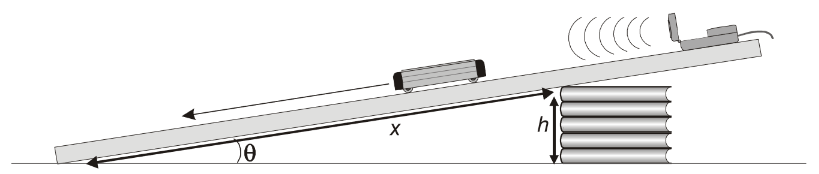
\includegraphics[width=\textwidth]{images/incline.png}
        \caption{Schiefe Bahn}
        \label{incline}
    \end{figure}

    \section{Vorfragen}
    \subsection{Experiment 1: Ball fallenlassen}
    Als erstes Experiment haben wir einen Ball aus \SI{2}{\metre} Höhe
    fallenlassen. Dabei haben wir die Zeit $t$, welche er bis zum Boden
    benötigt, gemessen.
    \subsubsection{Messung mit Herzfrequenz}
    In einem ersten Teil dieses Experiments haben wir $t$
    mithilfe unserer Herzfrequenz gemessen.
    Unseren Messungen zufolge
    braucht der Ball ungefähr gleich lang wie ein Herzschlag. Die
    durchschnittliche Herzfrequenz eines erwachsenen Menschen in unserem
    Alter und sportlichen Zustand beträgt 70 Schläge pro Minute (\SI{70}{\per\minute}).

    Berechnung der Zeit $t$ für einen Herzschlag:
    
    \begin{align}
        \Delta t &= \frac{n}{f} \label{tnf} \\
        \Delta t &= \frac{1}{\SI{1.17}{\per\second}} \\
        t &= \SI{0.86}{\second}
    \end{align}

    Zur Berechnung der Beschleunigung verwenden wir
    die Formel:

    \begin{align}
        s &= \frac{1}{2} \cdot a \cdot t^2 \\
        a &= \frac{2 \cdot s}{t^2} & \text{(Termumformung)} \label{ast}
    \end{align}

    Mit unseren gemessenen Werten erhalten wir somit:

    \begin{equation}
        a = \frac{2 \cdot \SI{2}{\metre}}{(\SI{0.86}{\second})^2}
        \approx \accunit{5.41}
    \end{equation}

    Dies ist etwa \accunit{4.4} zu klein. Dieser Fehler kommt
    einerseits von ungenauen Messmethoden (Herzfrequenz), andererseits
    von unserer Reaktionszeit. Ausserdem verfälscht der Luftwiderstand
    weiterhin das Resultat. Die korrekte Zeit, welche der Ball
    im Vakuum bräuchte, wäre ca. \SI{0.64}{\second}.

    \subsubsection{Messung mit Stoppuhr}
    Im zweiten Teil dieses Experiments haben wir die benötigte
    Zeit mit einer Stoppuhr gemessen. Wir erhielten dabei eine
    Zeit $t$ von \SI{360}{\milli\second}.

    Wenn wir diese Messung wieder der Formel aus (\ref{ast})
    mitgeben, erhalten wir eine Beschleunigung von:
    \begin{equation}
        a = \frac{2 \cdot \SI{2}{\metre}}{(\SI{0.360}{\second})^2}
        \approx \accunit{30.86}
    \end{equation}
    
    Dies ist wesentlich zu hoch. Dies ist zwar überraschend, 
    da wir eine wesentlich genauere Messmethode anwendeten,
    jedoch spielt unsere Reaktionszeit immernoch eine entscheidende
    Rolle. Wir haben einfach zu früh gestoppt oder die Stoppuhr
    zu spät gestartet.

    \subsection{Experiment: Ball auf schiefer Bahn}
    Für das nächste Experiment haben wir einen Ball von einer 
    schiefen Bahn herunterrollen lassen und die Zeit gemessen
    (siehe Abbildung \ref{incline}).

    \begin{tabular}{|l|l|}
        \hline
        $\theta$ & \SI{10}{\degree} \\
        x & \SI{1}{\metre} \\
        \hline
    \end{tabular}

    \subsubsection{Zeitmessung mit Herzfrequenz}
    Unseren Messungen zufolge benötigt der Ball ungefähr drei Herzschläge
    für einen Meter. Unter der Annahme, dass unsere durchschnittliche
    Herzfrequenz $f$ \SI{70}{\per\minute} ($\approx \SI{1.17}{\per\second}$) 
    beträgt, erhalten wir durch die Formel aus (\ref{tnf}):

    \begin{equation}
        t = \frac{3}{\SI{1.17}{\per\second}} \approx \SI{2.57}{\second}
    \end{equation}

    Anhand der Formel aus (\ref{ast}) erhalten wir für die Beschleunigung $a$
    bei einem Neigungswinkel von \SI{10}{\degree}:

    \begin{equation}
        a = \frac{2 \cdot \SI{1}{\metre}}{(\SI{2.57}{\second})^2} \approx \accunit{0.303}
    \end{equation}
    
    \subsection{Wie aussagekräftig sind diese Experimente?}
    Die Fehlerquellen sind natürlich sehr gross. Insbesondere zu Zeiten 
    Galileis waren die Messmöglichkeiten stark beschränkt und haben somit
    eine genaue Berechnung verhindert. Jedoch ermöglichen die Messungen
    immerhin einen Wert, an welchem man sich ungefähr orientieren konnte.
    Auch wenn er ungenau ist, ist es ein physikalischer Durchbruch, eine
    ungefähre Grössenordnung zu kennen.


    \section{Hauptexperiment: Schiefe Ebene}
    Wir haben unser Experiment wiederum eingerichtet, wie auf Abbildung
    \ref{incline} dargestellt. Dann haben wir verschiedene Objekte
    herunterrollen lassen mit verschieden Höhen
    \emph{h}. Die Länge \emph{x} ist die Distanz, in welcher
    wir die Objekte messen. Der Winkel $\theta$ bezeichnet
    den Winkel der schiefen Ebene.

    \subsection{Messung mit einem Ball}
    Zunächst haben wir einen Ball herunterrollen lassen.
    Sein Radius \emph{r} beträgt etwa 4 cm, seine Masse
    \emph{m} 242 g.
    
    Wir haben die Strecke $s$ in Abhängigkeit
    der Zeit $t$ gemessen, um die Beschleunigung
    $a$ zu bestimmen. Dazu haben wiederum die Formel
    aus (\ref{ast}) verwendet.
    Die Messwerte sind in der Tabelle \ref{ball}
    ersichtlich.

    \subsection{Messung mit einem Cart}
    Um die Reibung und den Luftwiderstand möglichst 
    klein zu halten und somit eine möglichst genaue
    Messung zu erzielen, haben wir das ganze Experiment
    auch mit einem Cart durchgeführt. Der Vorgang war
    prinzipiell derselbe, jedoch haben wir hohere
    Beschleunigungen erhalten, wie in Tabelle \ref{cart}
    dargestellt.



    \begin{table}
        \begin{tabularx}{\textwidth}{|X|X|X|X|X|X|X|}
            \hline
            \textbf{Number of books} & \textbf{Height of books $(m)$} & 
            \boldmath{$\sin{\theta}$} & \textbf{Trial 1}
            (\accunit{}) & 
            \textbf{Trial 2} (\accunit{}) & 
            \textbf{Trial 3} (\accunit{}) & 
            \textbf{Average acceleration} (\accunit{}) \\
            \hline
            3 & 0.115 & 0.0479 & 0.26 & 0.31 & 0.36 & 0.310 \\
            \hline
            4 & 0.144 & 0.0600 & 0.49 & 0.38 & 0.41 & 0.426 \\
            \hline
            5 & 0.174 & 0.073 & 0.60 & 0.45 & 0.38 & 0.476 \\
            \hline
            6 & 0.200 & 0.083 & 0.61 & 0.59 & 0.56 & 0.586 \\
            \hline
            7 & 0.275 & 0.115 & 0.97 & 1.22 & 1.22 & 1.137 \\
            \hline
        \end{tabularx}
        \caption{Messwerte (Ball)}
        \label{ball}
    \end{table}

    \begin{table}
        \begin{tabularx}{\textwidth}{|X|X|X|X|X|X|X|}
            \hline
            \textbf{Number of books} & \textbf{Height of books $(m)$} & 
            \boldmath{$\sin{\theta}$} & \textbf{Trial 1}
            (\accunit{}) & 
            \textbf{Trial 2} (\accunit{}) & 
            \textbf{Trial 3} (\accunit{}) & 
            \textbf{Average acceleration} (\accunit{}) \\
            \hline
            3 & 0.115 & 0.0479 & 0.70 & 0.864 & 0.68 & 0.748 \\
            \hline
            4 & 0.144 & 0.0600 & 0.83 & 0.93 & 0.83 & 0.863 \\
            \hline
            5 & 0.174 & 0.073 & 0.94 & 0.99 & 0.99 & 0.973 \\
            \hline
            6 & 0.200 & 0.083 & 1.43 & 1.33 & 0.93 & 1.23 \\
            \hline
            7 & 0.275 & 0.115 & 2.43 & 3.40 & 2.72 & 2.85 \\
            \hline
        \end{tabularx}
        \caption{Messwerte (Cart)}
        \label{cart}
    \end{table}


\end{document}